%**********************************************************
The remote system is responsible for the communication between the local systems and the internet. In this project, the internet is used to maintain a cloud database, so the remote system does the data bridge between the network of street lampposts and a cloud. 

%As one can see in figure \ref{fig:rs_overview}, the remote system is composed by the main process and a daemon process \textit{dServerSend}. The main process may be composed of a server and varoius clients, being the messages from each client received and processed in this process. The messages are sent to the clients in the daemon process \textit{dServerSend}. The communication between the two processes is done using message queues, so when a command is received and successfully parsed, the main process sends the command output to the daemon using the message queue.

%\begin{figure}[H]
%	\centering
%	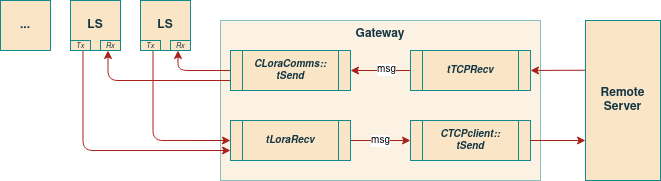
\includegraphics[width=.6\textwidth]{09sw_specification/RS/overview}
%	\caption{Inter-process Communication between Main Process and Daemon.}
%	\label{fig:rs_overview}
%\end{figure}

%**********************************************************
\subsection{Class Diagram}
In figure \ref{fig:rs_classDiag} is represented the class diagram of the remote system. The class \textit{CRemoteSystem} is the main class of this system, that initializes the objects of each class, listed below. As members, this class has a server, \textit{CTCPServer}, a list of connected clients, \textit{CClients}, and a database, \textit{CDataBase}. 

\begin{itemize}
	\item \textbf{CTCPServer:} responsible for creating the server and accepting the clients connections;
	\item \textbf{CClient:} client class, stores the clients information, receives their messages, executing the respective command and sends its output to the client;
	\item \textbf{CDataBase:} provides an interface between the server and the database.
\end{itemize}

\begin{figure}[H]
	\centering
	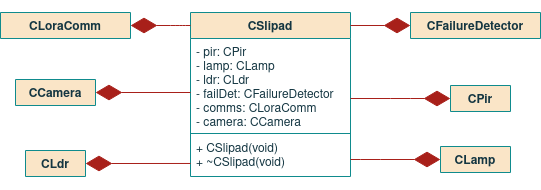
\includegraphics[width=.9\textwidth]{09sw_specification/RS/ClassDiagram}
	\caption{Remote System Class Diagram.}
	\label{fig:rs_classDiag}
\end{figure}


%****************************
\myparagraph{Class CTCPServer}

This class is responsible for creating the server, using \textit{createServer} method. Furthermore, using the function \textit{acceptConnection}, this class accepts the clients connections returning the socket file descriptor. This class contains the information about the server address, \textit{addr}, the listen socket descriptor, \textit{listenSd} and the maximum number of connected clients, \textit{maxClients}. In figure \ref{fig:CTCPServer}, one can see the class \textit{CTCPServer} diagram.

\begin{figure}[H]
	\centering
	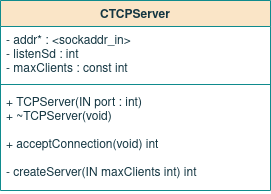
\includegraphics[width=.6\textwidth]{09sw_specification/RS/CTCPServer/CTCPServer}
	\caption{Class Diagram: CTCPServer.}
	\label{fig:CTCPServer}
\end{figure}

%****************************
\myparagraph{Class CClient}

The class \textit{CClient}, represented in figure \ref{fig:CClient}, is responsible for storing information about a client connected to the remote system, like the \textit{cmdList}, a vector that stores the commands list that the client can execute and \textit{clientSock}. The \textit{clientSock} has information about the client like its \textit{state}, \textit{name}, identification number, \textit{index}, sock file descriptor, \textit{sockFd} and \textit{type}, that can be \textit{APPLICATION}, for a mobile application client, \textit{WEBSITE}, for a web site client or \textit{GATEWAY}, for a gateway device client. Furthermore, this class inherits from the class \textit{CCommunication}, that implements the mechanism of sending messages to the client, and implements the thread to receive and parse messages from the client, \textit{tRecv}. 

\begin{figure}[H]
	\centering
	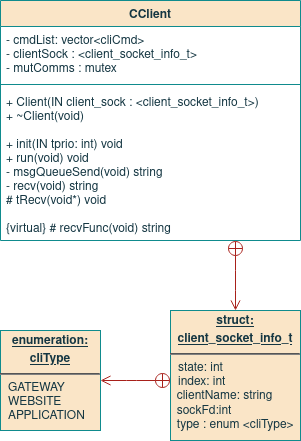
\includegraphics[width=.9\textwidth]{09sw_specification/RS/CClient/CClient}
	\caption{Class Diagram: CClient.}
	\label{fig:CClient}
\end{figure}

%****************************
\myparagraph{Class CDataBase}

%This class diagram is shown in figure \ref{fig:CDataBase}, and is responsible for implement the interface between the server and the database, having for that a pointer to a database of type \textit{MYSQL}. To interact with the database, the server must first prepare a query, using the function \textit{prepareQuery}, and can update or get data from the database, using the prepared query and the functions \textit{updateData} and \textit{getData}, respectively.

\begin{figure}[H]
	\centering
	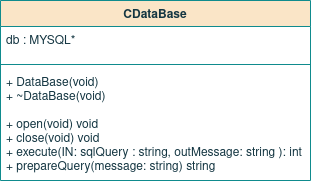
\includegraphics[width=.5\textwidth]{09sw_specification/RS/CDataBase}
	\caption{Class Diagram: CDataBase.}
	\label{fig:CDataBase}
\end{figure}

%**********************************************************
\subsection{Task Overview}
One can define and describe briefly how the remote system is implemented, making use of threads and processes. 

\begin{itemize}
	\item \textbf{tSend:} sends a message to the client;
	\item \textbf{tRecv:} receives a message from the client.
\end{itemize}

%**********************************************************
\subsection{Task Priority}
The priority assignment for the remote system is shown in figure \ref{fig:rsPrio}. The thread \textit{tRecv} has a higher priority than the thread \textit{tSend} because one never knows when a client is going to send a message. 

\begin{figure}[H]
	\centering
	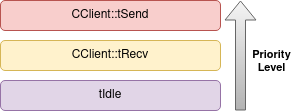
\includegraphics[width=.5\textwidth]{09sw_specification/RS/ThreadsPrio}
	\caption{Remote System Main Process Priority Assignment.}
	\label{fig:rsPrio}
\end{figure}

%**********************************************************
\subsection{Task Synchronization}
As seen before, to have coordinate access to shared ressouces and services and avoid race conditions, the kernel has resources that provide synchronization between the tasks. 

\myparagraph{Mutexes}

The mutexes used for the remote system are listed bellow.

\begin{itemize}
	\item \textbf{CCommunication::mutComms:} already detailed in the local system section; used in-directly by \textit{CClient}; used to protect the communications;
	\item \textbf{CCommunication::mutTxMsgs:} already detailed in the local system section; used in-directly by \textit{CClient}; used to protect the insertion and removal of messages into \textit{TxMsgs};
\end{itemize}

\myparagraph{Condition Variables}

The condition variables used for the remote system are listed bellow.

\begin{itemize}
	\item \textbf{CCommunication::condSend:} already detailed in the local system
	section; this condition variable is used indirectly by \textit{CClient}; used to notify CCommunication::tSend that a new message is ready to be sent.
\end{itemize}

%\subsection{Task Communication}
% Nothing to show here

%**********************************************************
\subsection{Start-up Process}
The start-up process is shown in the figure \ref{fig:RSstart}. When the program initiates, the start-up process instantiate a object of the class \textit{CRemoteSystem}. After that, it uses the method \textit{run} that will be seen in the next subsection.

\begin{figure}[H]
	\centering
	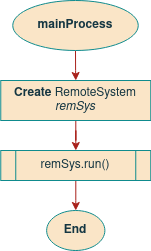
\includegraphics[width=0.3\textwidth]{09sw_specification/RS/start}
	\caption{Start-Up Process.}
	\label{fig:RSstart}
\end{figure}

%**********************************************************
\clearpage
\subsection{Flowcharts}
%********************************
\myparagraph{CRemoteSystem}

The figure \ref{fig:rsConst} represents the \textit{CRemoteSystem} class's constructor that is responsible for the creation of the \textit{clientList} vector, the database object, \textit{db} and the server \textit{server} in the port passed by argument.

\begin{figure}[H]
	\centering
	\includegraphics[width=.26\textwidth]{09sw_specification/RS/CRemoteSys/Const}
	\caption{Flowchart: CRemoteSystem Constructor.}
	\label{fig:rsConst}
\end{figure}

In figure \ref{fig:rsRun} is shown the \textit{CRemoteSystem} run method. Is is used to, after the creation of the server socket, accept the connections coming from the clients, using the \textit{CTCPServer} method to accept connections, \textit{acceptConnection}, that returns the socket descriptor of the new connection. If the socket descriptor \textit{sd} is valid, then it is created a client \textit{CClient} with this variable and the client is inserted in the client vector, \textit{clientList}.

\begin{figure}[H]
	\centering
	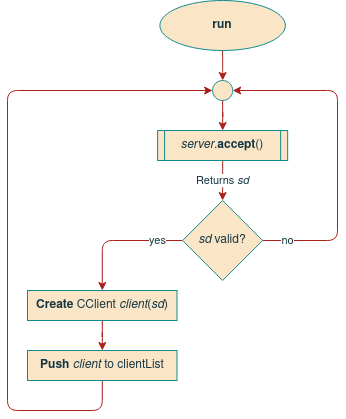
\includegraphics[width=.6\textwidth]{09sw_specification/RS/CRemoteSys/Run}
	\caption{Flowchart: CRemoteSystem run.}
	\label{fig:rsRun}
\end{figure}

%********************************
\myparagraph{CTCPServer}

In figure \ref{fig:ServerConst} is represented the constructor of the \textit{CTPCServer} class, that is responsible for creating the server socket in the port passed by argument, using the function \textit{createServer}.

\begin{figure}[H]
	\centering
	\includegraphics[width=.26\textwidth]{09sw_specification/RS/CTCPServer/Const}
	\caption{Flowchart: CTCPServer Constructor.}
	\label{fig:ServerConst}
\end{figure}

The function that creates a server socket for a maximum number of clients, \textit{maxClient}, is represented in figure \ref{fig:RSCreateServer}. This function create a server socket with the IPv4 protocol connection, initialize the \textit{addr} with the port number passed by argument, binds the socket and listen to a maximum number of clients connections specified by \textit{maxClient} passed by argument.

\begin{figure}[H]
	\centering
	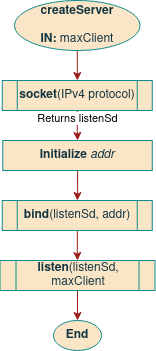
\includegraphics[width=.25\textwidth]{09sw_specification/RS/CTCPServer/CreateServer}
	\caption{Flowchart: CTCPServer createServer.}
	\label{fig:RSCreateServer}
\end{figure}

In figure \ref{fig:acceptConn} is represented the \textit{acceptConnection} method, that accepts a connection from a client in the socket referenced by the socket file descriptor \textit{listenSd}, returning the file descriptor of the new connection, \textit{sd}.

\begin{figure}[H]
	\centering
	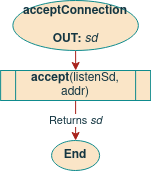
\includegraphics[width=.25\textwidth]{09sw_specification/RS/CTCPServer/acceptConnection}
	\caption{Flowchart: CTCPServer acceptConnection.}
	\label{fig:acceptConn}
\end{figure}

%**********************************
\myparagraph{CClient}

In figure \ref{fig:ClientConst} is represented the constructor of the \textit{CClient} class. Every time a client connects to the remote system, it creates an instance of this class, passing by argument, the information about the client to initialize the \textit{clientSock} variable. The constructor also creates the command list that the type of client can execute, \textit{cmdList}, and the threads \textit{tRecv} and \textit{tSend}, using the method \textit{initThFun}.

\begin{figure}[H]
	\centering
	\includegraphics[width=.20\textwidth]{09sw_specification/RS/CClient/Const}
	\caption{Flowchart: CClient Constructor.}
	\label{fig:ClientConst}
\end{figure}

!!!!!!!!!!!!!!!!!!!!!!!!!!!!!!!!!!!!!!!!!!!!!!!!!!!!!!!!!!!!!!!!!!!!!
!!!!!!!!!!!!!!!!!!!!!!!!!!!!!!!!!!!!!!!!!!!!!!!!!!!!!!!!!!!!!!!!!!!!!
The command list, \textit{cmdList} varies with the type of client:

\begin{itemize}
	\item \textbf{Mobile Application:} 
		\begin{itemize}
			\item Get;
			\item Update;
			\item Delete.
		\end{itemize}
	
	\item \textbf{Web Site:}
		\begin{itemize}
			\item Get.			
		\end{itemize}
	
	\item \textbf{Gateway:}
		\begin{itemize}
			\item Get;
			\item Update.
		\end{itemize}

\end{itemize}

In the method \textit{initThFun}, shown in figure \ref{fig:clientInit}, it is created the thread \textit{tRecv} with priority \textit{recvPrio}, that receives messages from the clients, and the thread \textit{tSend} with priority \textit{sendPrio}, that is implemented in the class \textit{CCommunication} and sends messages to the clients.

\begin{figure}[H]
	\centering
	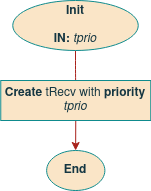
\includegraphics[width=0.26\textwidth]{09sw_specification/RS/CClient/init}
	\caption{Flowchart: CClient initThFun.}
	\label{fig:clientInit}
\end{figure}

The method \textit{runThFun}, represented in figure \ref{fig:clientRun}, is responsible for waiting for the termination of the threads \textit{tRecv} and \textit{tSend}.

\begin{figure}[H]
	\centering
	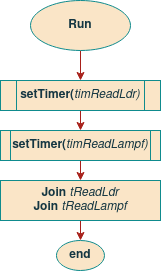
\includegraphics[width=0.26\textwidth]{09sw_specification/RS/CClient/run}
	\caption{Flowchart: CClient runThFun.}
	\label{fig:clientRun}
\end{figure}

The figure \ref{fig:RSRecv} shows the thread that receive messages from the clients, \textit{tRecv}. When a message is received, the function \textit{recv} returns the received message. If it is not empty, then one can parse and execute the command extracted from the received message, using the \textit{parseExecute} function. When the command is valid, this function returns a message to be sent back to the client. In order to send this message to the client, one needs to use the \textit{CCommunication} method to push this message to the sending buffer.

\begin{figure}[H]
	\centering
	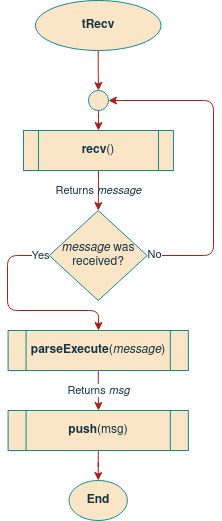
\includegraphics[width=0.4\textwidth]{09sw_specification/RS/CClient/tRecv}
	\caption{Flowchart: CClient tRecv.}
	\label{fig:RSRecv}
\end{figure}

%In figure \ref{fig:parseExecute} is represented the flowchart of the \textit{parseExecute} function, that is responsible for parsing and execute the message sent by the client. It is needed to verify if the client that sent the command has rights to execute that command, so the message sent is searched in the \textit{cmdList} assigned to the respective client. If the message corresponds to a valid command for that client, then one can prepare a query and execute the command according to the type of command that was sent: \textit{delete} for a data deletion, \textit{update} for a data update and \textit{get} for a data request, returning the command output in a string message \textit{msg}. If the command doesn't exist in the command list of that client, then the \textit{msg} is assigned with an error message. The output of this function is the string message, \textit{msg}.

In figure \ref{fig:parseExecute} is represented the flowchart of the \textit{parseExecute} function, that is responsible for parsing and execute the message sent by the client. It is needed to verify if the client that sent the command has rights to execute that command, so the command sent is searched in the \textit{cmdList} assigned to the respective client. If the message corresponds to a valid command for that client, then one can execute the command. If the command doesn't exist in the command list of that client, then the \textit{msg} is assigned with an error message. The output of this function is the string message to be sent back to the client, \textit{msg}.

\begin{figure}[H]
	\centering
	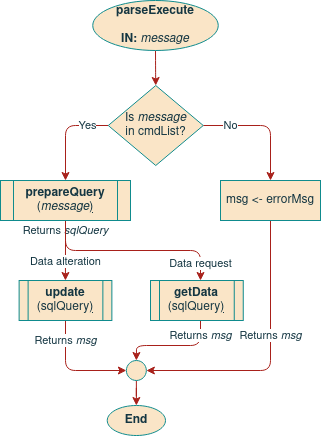
\includegraphics[width=0.6\textwidth]{09sw_specification/RS/CClient/parseExecute}
	\caption{Flowchart: CClient parseExecute.}
	\label{fig:parseExecute}
\end{figure}

As for the previous subsystems, this class must implement the \textit{recvFunc} and \textit{sendFunc} methods, as they are pure virtual methods from CCommunication. 

In this class, one will use existent functions \textit{TCPReceive} and \textit{TCPSend} to implement TCP-IP communication, as shown in figures \ref{fig:RSrecvfunc} and \ref{fig:RSsendfunc}. This functions make use of the socket created when the TCP-IP connection was established.

\begin{figure}[H]
	\centering
	\includegraphics[width=.35\textwidth]{09sw_specification/RS/CClient/Recvfunc}
	\caption{Flowchart: CClient recvFunc method.}
	\label{fig:RSrecvfunc}
\end{figure}

\begin{figure}[H]
	\centering
	\includegraphics[width=.35\textwidth]{09sw_specification/RS/CClient/Sendfunc}
	\caption{Flowchart: CClient sendFunc method.}
	\label{fig:RSsendfunc}
\end{figure}